\begin{figure}
\centering
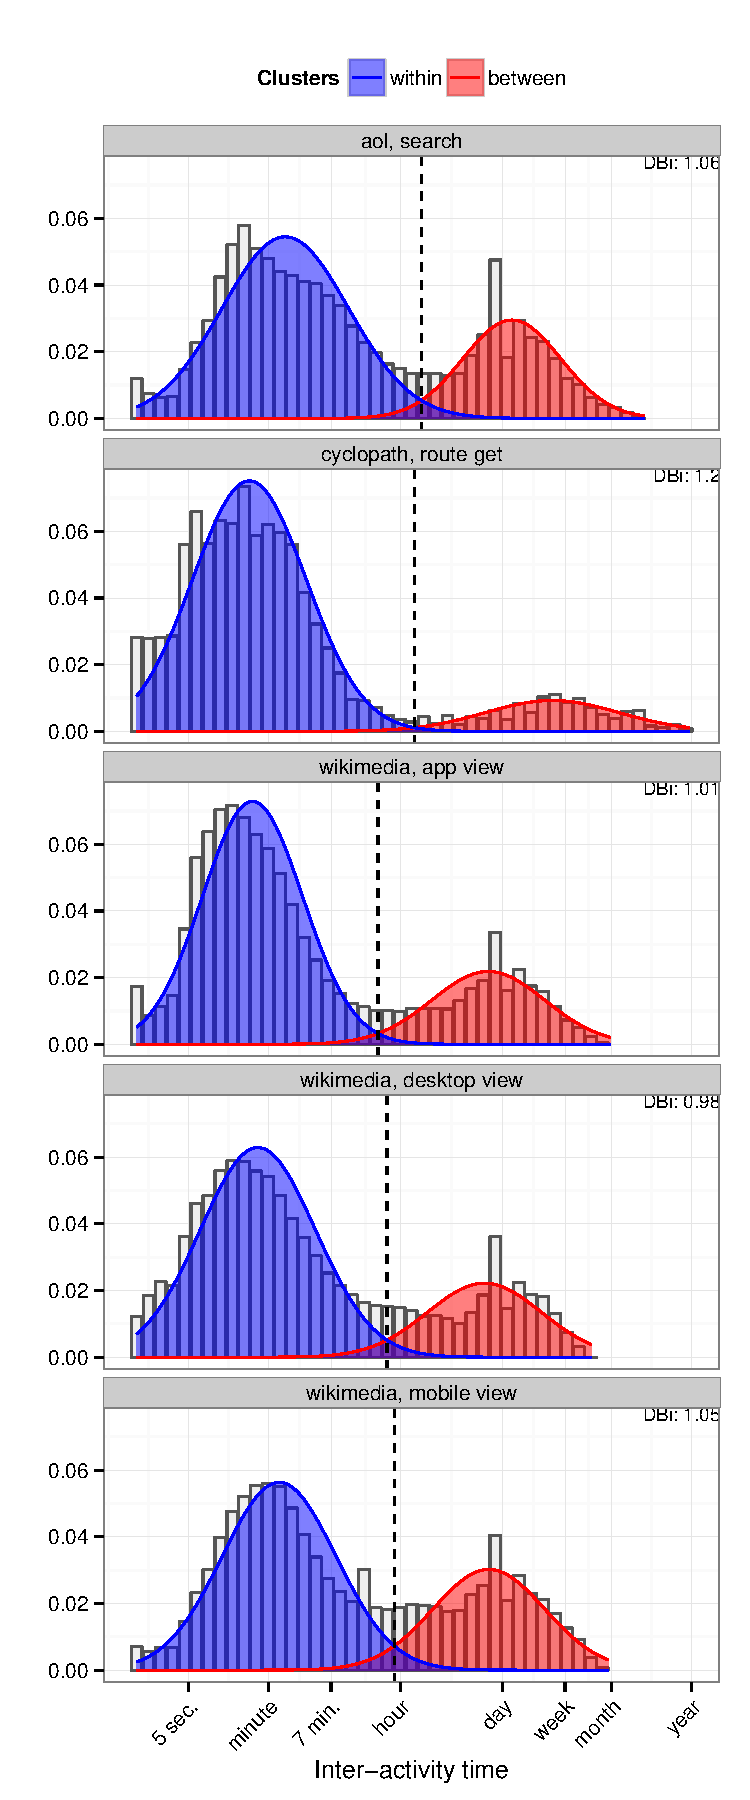
\includegraphics[width=.45\textwidth]{figures/bimodal_clusters.pdf}
\label{fig:bimodal_clusters}
\caption{
    \textbf{Bimodal clusters.} Empirical inter-activity density (bars) and fitted mixture models of gaussians are plotted for datasets where two clusters appeared to sufficiently explain the observed data.
}
\end{figure}
\begin{table*}
\label{tab:fits}
\centering
\caption{Fit and threshold information for clusters.  Note that fits correspond to logarithmically scaled (base 2) seconds between events.  For example, $2^{6.7} = 104 \text{ seconds}$.  It's important to report these values in log scale because, while the mean can be re-exponentiated, the standard deviation of log values doesn't make sense that way. }
\begin{tabular}{|r|r|r|r|r|r|r|r|r|r|r|r|r|r|} \hline
\multirow{2}{*}{\textbf{dataset}} &
\multirow{2}{*}{\textbf{theshold (min)}} &
\multicolumn{3}{|c|}{\textbf{short within}} &
\multicolumn{3}{|c|}{\textbf{within}} &
\multicolumn{3}{|c|}{\textbf{between}} &
\multicolumn{3}{|c|}{\textbf{break}} \\ \cline{3-14}
& &
                           $\mu$       & $\sigma$   & $\lambda$
                         & $\mu$       & $\sigma$   & $\lambda$
                         & $\mu$       & $\sigma$   & $\lambda$
                         & $\mu$       & $\sigma$   & $\lambda$\\ \hline
aol search    & 115      &&&
                         & 6.7         & 2.9         & 0.70
                         & 16.8        & 2.2         & 0.30&&&\\ \hline
cyclo. route  & 89       &&&
                         & 5.0         & 2.5         & 0.87
                         & 18.6        & 3.1         & 0.13&&&\\ \hline
wiki. app     & 29       &&&
                         & 5.2         & 2.3         & 0.74
                         & 15.7        & 2.5         & 0.26&&&\\ \hline
wiki. mobile  & 50       &&&
                         & 6.4         & 2.6         & 0.65
                         & 15.8        & 2.5         & 0.35&&&\\ \hline
wiki. desktop & 46       &&&
                         & 5.5         & 2.6         & 0.75
                         & 15.7        & 2.5         & 0.25&&&\\ \hline
osm change    & 101      &&&
                         & 8.6         & 2.1         & 0.68
                         & 15.5        & 2.5         & 0.30
                         & 22.7        & 2.0         & 0.02\\ \hline
wiki. edit    & 80       &&&
                         & 6.8         & 2.5         & 0.83
                         & 15.4        & 2.7         & 0.16
                         & 22.6        & 1.9         & 0.01\\ \hline
mov. rating   & 33       & 3.0         & 1.3         & 0.58
                         & 5.2         & 1.9         & 0.34
                         & 18.0        & 3.0         & 0.07&&&\\ \hline
mov. search   & 52       & 4.0         & 0.8         & 0.30
                         & 5.7         & 2.5         & 0.50
                         & 17.1        & 3.1         & 0.20&&&\\ \hline
lol game      & 14       &&&
                         & 8.3         & 0.5         & 0.59
                         & 14.1        & 2.8         & 0.41&&&\\ \hline
s. o. answer  & 91       &&&
                         & 10.2        & 1.7         & 0.30
                         & 16.6        & 2.9         & 0.63
                         & 23.0        & 1.5         & 0.06\\ \hline
s. o. quest.  & 335      &&&
                         & 12.7        & 1.7         & 0.10
                         & 18.5        & 2.1         & 0.63
                         & 22.4        & 1.7         & 0.26\\ \hline

\end{tabular}
\end{table*}

In this section, we present and discuss the result of the application of our proposed inactivity threshold identification analysis on the datsets.  First we start off with the common, simple cluster fits.  Then we move to more complicated fits and discuss the implications of additional clusters,  Finally, we demonstrate datasets with less suitable fits and discuss what this implies about the nature of participation in these systems.

\subsection{Simple bimodal fits}
Most of the datasets of user-initiated inter-activity times that we observed display a simple bimodal distribution when their histograms are plotted on a logarithmically scaled X axis.  Figure \ref{fig:bimodal_clusters} plots a log inter-activity time histogram overlaid with expectation maximization fits of a mixture of two log-normal cluster components.  Notably, the AOL search logs represent one of the most clear fits to this bimodal distribution.  This suggests that, counter to Mehrzadi
\& Feitelson's conclusions\cite{mehrzadi2012onextracting}, there does seem to to be a clear location for an inactivity cutoff in this dataset -- at approximately one hour.

Figure \ref{fig:bimodal_clusters} demonstrates the striking regularity of inter-activity time between systems.  All of the systems presented show a clear fit for a theoretical \emph{within-session} cluster with a mode around 1 minute and a theoretical \emph{between-session} cluster with a mode at 1 day.  Each fit intersects at approximately one hour -- with Wikimedia app views display the lowest intersection at 29 minutes while AOL searches display the highest intersect at 115 minutes -- nearly two hours.   Despite this variance in the intersection points, a visual inspection of the empirical distribution does not suggest that the choice of a 1 hour cutoff for either of these datasets would be inappropriate.  Indeed, many of the \emph{between-session} clusters appear to be left shifted due to a lack of longitudinal data and it is only in these cases that the intersection falls below the one hour mark.

Also of note in these results is the spike of probability of a 24 hour inter-activity time for all but the cyclopath datasets.  This suggests that, for reading Wikimedia sites and searching in AOL, there is a strong tendency to return on a daily basis.  The curious lack of such a day-spike for cyclopath route searches could be explained by the type of usage the site sees. Bicycle route searching may be less of a daily information need than web search and Wikimedia's encyclopedia content.

\subsection{Fits with extended breaks}
\begin{figure}
\centering
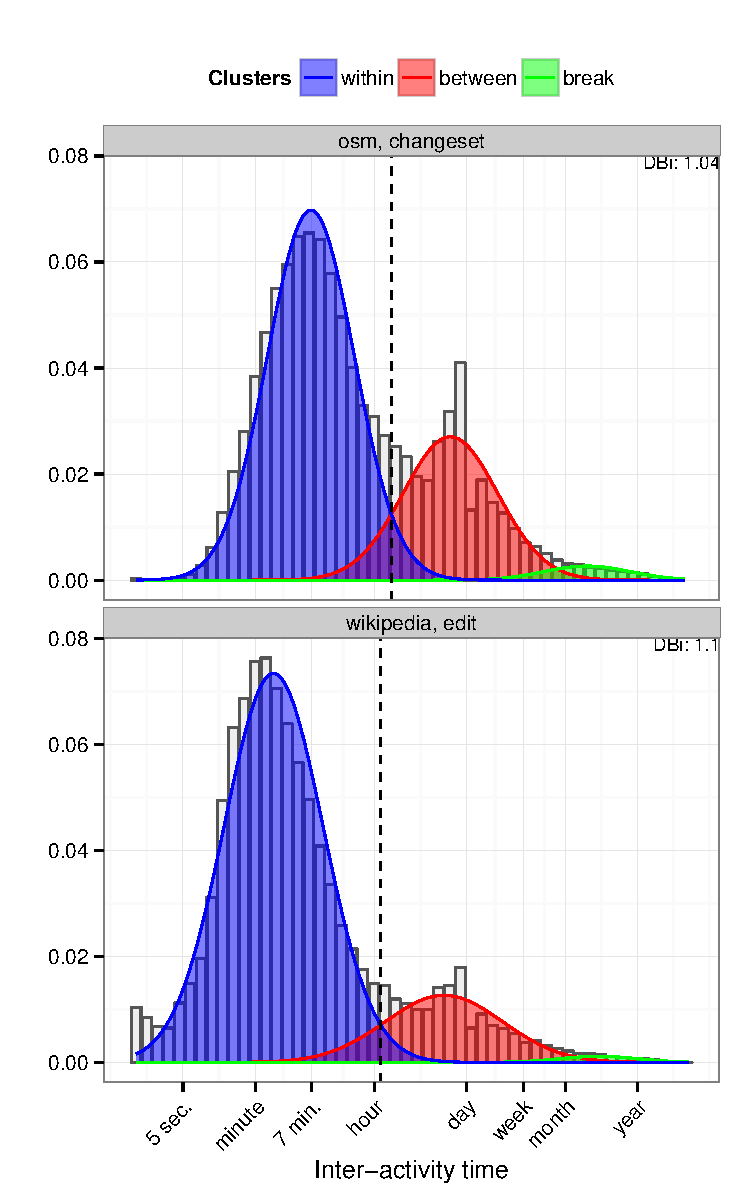
\includegraphics[width=.45\textwidth]{figures/trimodal_clusters.pdf}
\label{fig:trimodal_clusters}
\caption{
    \textbf{Trimodal clusters.} Empirical inter-activity density (bars) and fitted mixture models of gaussians are plotted for datasets where an additional, ``break'' cluster was needed to fit the data.
}
\end{figure}
In some cases, we found that the data were fit better by adding a third component to the mixture model that represents very low frequency events.  Figure \ref{fig:trimodal_clusters} shows the fits for the inter-activity time between Open Street Map's changesets and English Wikipedia edits.  Note that, like the bimodal fits above, we again see modes for the \emph{within-session} cluster around 1 minute and modes for the \emph{between-session} cluster around 1 day.  However, we found that we could more cleanly fit these datasets with an additional cluster with a mode of around 2.5 months.

As we noted in \cite{geiger13using}, we believe that this low frequency cluster represents an extended break from contributing that corresponds to a life event -- like getting married, buying a house, going to school or getting a job.  Wikipedia editors refer to this phenomena in volunteer participation as a ``wikibreak''\footnote{\url{https://en.wikipedia.org/wiki/Wikipedia:Wikibreak}}.  We suspect that the reason for the tiny scale of this cluster is two-fold: (1) contributors who work on Wikipedia or Open Street Map for long enough to to take an extended break are rare compared to other, higher frequency activity and (2) breaks often result in total abandonment of participation in the project.

\subsection{Fits with a high frequency component}
When observing the distribution of inter-activity times for ratings and searches in Movielens, we found that both these events occurred with higher frequency than the other datasets.  This made us suspect that there could be an additional cluster component at a high frequency time interval.  Figure \ref{fig:operation_mixed_clusters} shows how the two datasets lent themselves to this additional ``short within'' component.  Like in previous mixture models, we see a within-session cluster with a mode around one minute and a between-session cluster with a mode around 1 day.  However, in these datasets we also observed a pattern in inter-activity times that suggested a faster component with a mode around 30 seconds.

Given that this component occurs at shorter intervals than the within-session component, we assume that it also represents within-session activity.  In the case of rating, this high frequency component could represent the rapid rating behavior that the Movielens interface affords -- a user can rate several movies from a list without leaving a page.  However, we're less sure of on how to explain the high frequency component of Movielens searches.  It could be that, unlike when performing a web search (AOL) or reading encyclopic content (Wikimedia), users' movie searches are more likely to benefit from more rapid iteration.
\begin{figure}
\centering
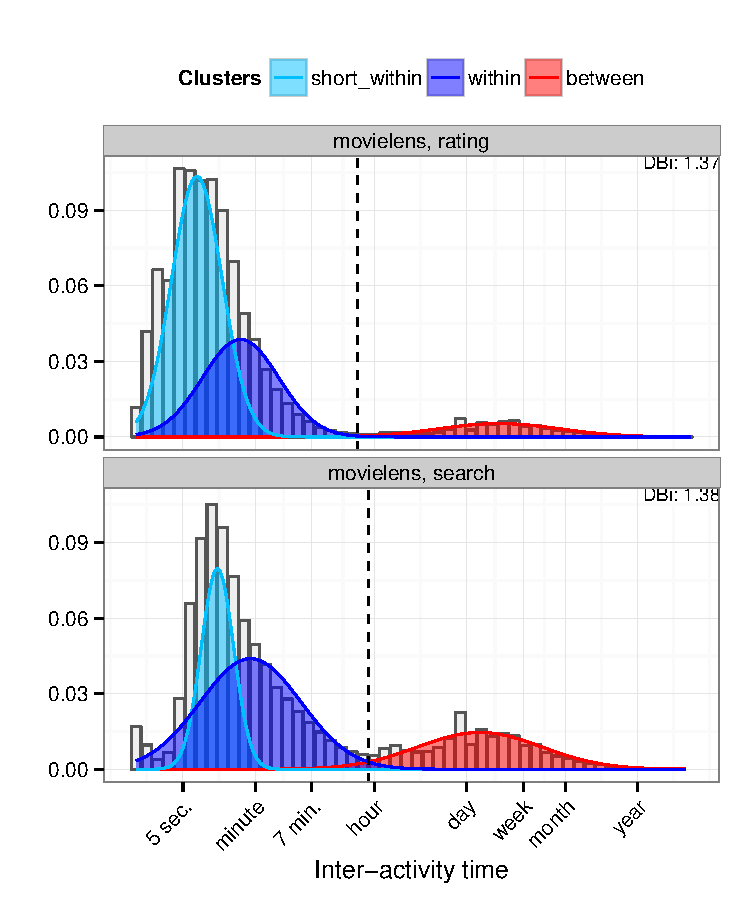
\includegraphics[width=.45\textwidth]{figures/operation_mixed_clusters.pdf}
\label{fig:operation_mixed_clusters}
\caption{
    \textbf{High frequency activity clusters.} Empirical inter-activity density (bars) and fitted mixture models of gaussians are plotted for datasets where an additional, high-frequency inter-activity cluster was needed to fit the data.
}
\end{figure}

\subsection{Unusual fits}
\begin{figure}
\centering
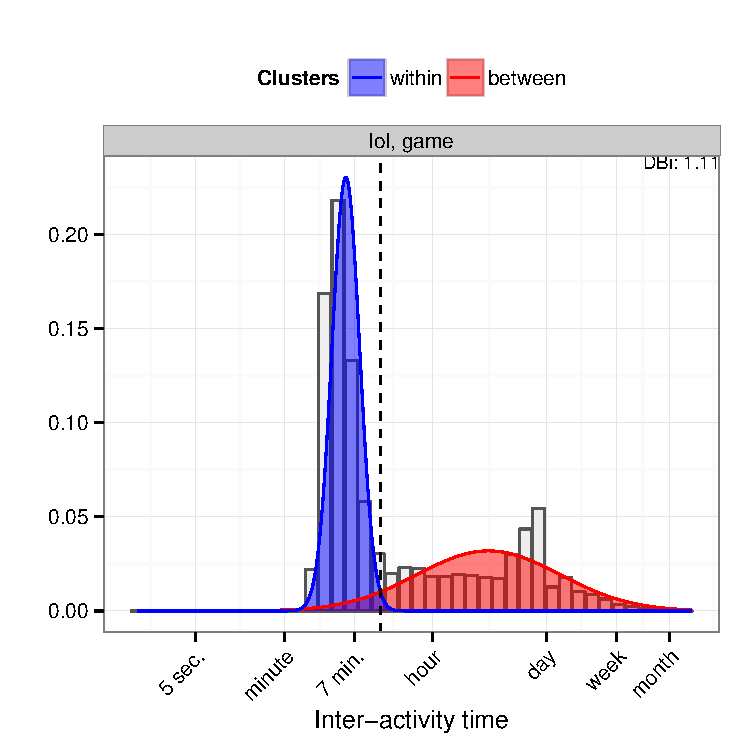
\includegraphics[width=.45\textwidth]{figures/weird_lol_clusters.pdf}
\label{fig:lol_game_clusters}
\caption{
    \textbf{Inter-game clusters.} Empirical inter-activity density (bars) and fitted mixture models of gaussians are plotted for time between League of Legends games.
}
\end{figure}
While the fits described so far follow a clear pattern with somewhat minor nuance as to the nature of the gaussian fitting strategy, the other datasets we observed suggest that the this strategy for identifying session thresholds is not universally suitable for all user-intiated events.

\leadin{League of Legends}
Figure \ref{fig:lol_game_clusters} shows the two cluster fit for League of Legends game playing.  Here, we see a very high density component with a mode around 5 minutes and a very wide component with a mode around 5 hours.  The intersection of these components place the threshold at approximately 14 minutes.  It is important to note that the tightness of the dense component may be an artifact of the way that inter-game times differ from the inter-activity times observed in the other datasets.  In the case of this dataset, only the time between games is accounted for -- not the time between game-start or game end.

There also may be constraints inherent to the system which limit the potential time spans in which a user could possibly act.  For example, League of Legends employs a queuing mechanism for matching teammates which takes approximately 5 minutes to complete at most times.  Our own experience with the game suggests that many users will finish one game and immediately get into the queue for another.  It is likely that these system limitations are the reason for infrequent between-game times under 1 minute, and understanding how systems limit user behavior is often helpful when interpreting cluster fit.

\leadin{Stack overflow}
\begin{figure}
\centering
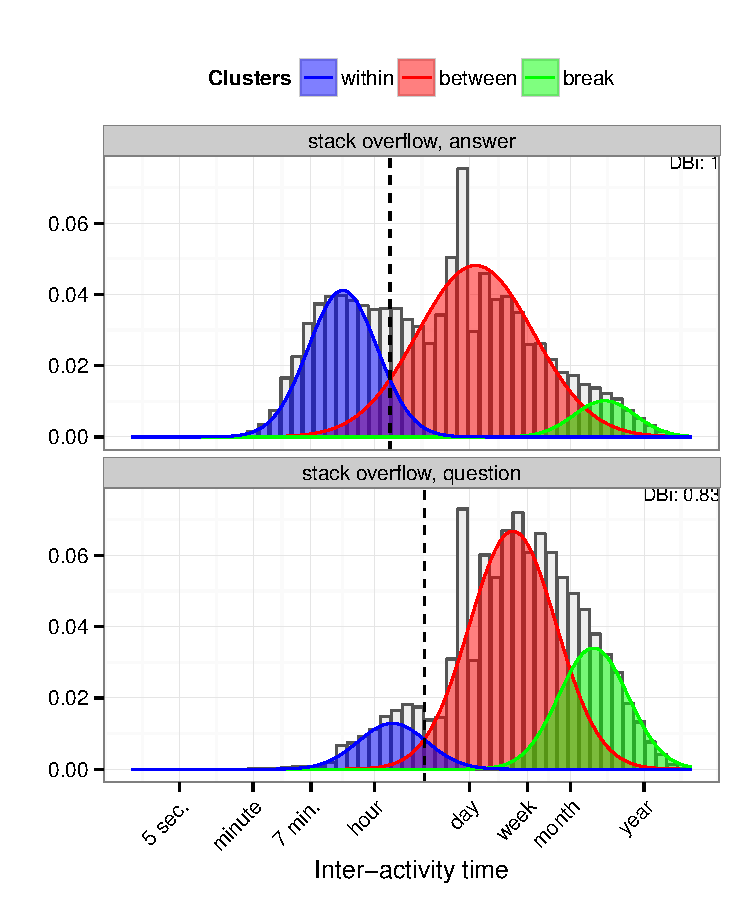
\includegraphics[width=.45\textwidth]{figures/weird_so_clusters.pdf}
\label{fig:stack_overflow_clusters}
\caption{
    \textbf{Low frequency clusters.} Empirical inter-activity density (bars) and (non-convergent) fitted mixture models of gaussians are plotted for time between posts on Stack Overflow.
}
\end{figure}
Unlike the other datasets observed, the time between Stack Overflow posts does not suggest a clear valley from which to draw intuition about where to draw a session cutoff.  Figure \ref{fig:stack_overflow_clusters} shows the (non-convergent) fits of question asking and answering activities.  In this case, there is a dramatic reduction in the scale of the higher frequency time components and what appears to be a shift of the within-session component to the right.

If we are to interpret the fit of these clusters as meaningful, the right shift of the within-session component could be due to the time needed to produce a high quality question or answer.  Stack Overflow's incentive structure is designed to encourage high quality posts.  High quality posts are more likely to be reviewed positively by other users, and a user's score within StackOverflow is largely dependent on how other users rate the quality of their posts\footnote{\url{http://meta.stackexchange.com/help/whats-reputation}}.  It's seems likely that producing a high quality post would take a substantial amount of time and that this time investment would make posting with a high enough frequency to produce a short inter-activity time component like we saw in other systems difficult.  In this case, it seems that either our strategy for identifying a suitable inactivity threshold is insufficient or that Stack Overflow users rarely post more than one question or answer within an activity session.
